%TODO One paragraph (3 sentences) on bikesharing having become ubiquitous, NYC being the largest systems in the US and rebalancing being the major operational challenge. Explain that full stations stop customers from returning, empty stations from renting -- both suck.
Bike-sharing systems have become ubiquitous in many American cities. The largest of these systems consist of a number of stations placed densely within a city; each station consists of a number of docks that each either hold a bike (are full) or are empty. Users can rent a bike from any station with at least one bike and return bikes at any station with an empty dock. With more than 30 million annual rides nationwide (2017), about half of which occurred in New York City's Citi Bike system, these systems have become a fixture of urban life, providing commuters and tourists with a sustainable transportation option.

The major operational challenge faced by these systems is to avoid out-of-stock events: as each station has a finite number of docks (\emph{capacity}) at which users can rent or return bikes, users are unable to enter the system when trying to rent bikes at stations at which all docks are empty, that is, when no dock holds a bike; arguably even worse, customers are not able to leave the system when they try to return bikes at stations at which all docks are full. In the past few years, researchers and system operators alike have developed tools to tackle such out-of-stock events and their underlying cause: \emph{imbalance}. This is often referred to as \emph{rebalancing}: moving bikes within the system to reduce the number of out-of-stock events. Rebalancing can be of various modes: for example, systems operate box trucks, pedicab trailers, and valet services to reduce out-of-stock events. In this paper, we describe our work with the operators of Citi Bike in setting up \emph{Bike Angels}, a crowdsourcing approach to rebalancing, and analyze the relative effectiveness of a variety of natural incentive schemes for their system.

The Bike Angels incentive scheme was first set up in October 2015. In the initial set-up, we identified pairs of stations that (i) were close to each other, and (ii) had asymmetric demand patterns: we chose pairs of stations that were nearby to each other but over a certain time interval had the property that one station (A) overwhelmingly had bikes returned whereas the other (B) overwhelmingly had bikes rented. We then invited users that often used one of the two and asked them to switch to the other, i.e., we asked a small number of customers likely to return bikes at A in such intervals to become \emph{Bike Angels} by instead returning bikes at~B. Of course, in such a scheme, incentives can only be used for a tiny fraction of rides within the system.

Nevertheless, the pilot showed that customer behavior could be significantly affected through gamification \cite{citibikeInternal}, and also posed questions about how to optimally design such an incentive scheme, in particular with respect to when and where to incentivize. A second version of Bike Angels, at a much larger scale, statically incentivized a sizeable fraction of stations within the system either to enourage rentals or returns throughout each rush hour.
This program was viewed as a great success, in spite of the fact that the pre-determined incentives made no use of the vast amounts of historic and real-time data available. At worst, this sometimes led to incentives  encouraging customers to rent (return) bikes at empty (full) stations. % about which station is labeled as what were made long ahead of time, we could not guarantee that stations that are usually in need of bikes at particular times would not end up full at those times (or vice-versa for stations usually overfilled with bikes).

In this paper, we evaluate the efficiency of this incentive scheme with regard to its goal to reduce out-of-stock events.  We apply so-called \emph{user dissatisfaction functions} to evaluate, for every trip rewarded by the program, an estimate of its reduction in future out-of-stock events. Further, we design a range of different policies, dictating the times at which each station is incentivized. The design of these policies involves trade-offs between their \emph{efficiency} and \emph{simplicity}. Below, we explain what we mean by those two terms:

\noindent \textbf{Efficiency.} The main goal of \emph{Bike Angels} is to help rebalance the system, i.e., to reduce the number of out-of-stock events. We explain in subsequent sections how the user dissatisfaction functions introduced by Raviv and Kolka  \cite{raviv2013optimal} can be used to evaluate the impact of each individual rental/return on the expected number of future out-of-stock events. Combining these with a cost for each point awarded in the incentive scheme, we obtain a score for each incentivized rental/return that can be interpreted as an offline evaluation of the efficiency of the incentive. In that sense, a perfectly efficient scheme would incentivize exactly those trips that net a positive score when accounting for both the impact on out-of-stock events and the cost of incentives.

\noindent \textbf{Simplicity. } Perfect efficiency, with respect to the score described above, is attainable in such an incentive scheme, but it requires the operator to decide in real-time whether or not to incentivize at each location. This is undesirable from the users' perspective as it reduces predictability on where incentives will be given in the future, i.e., when customers prepare their trip, they do not know whether or not their origin and, even more so, their destination has rentals and respectively, returns, incentivized. This raises the bar for participation. Further, from an operator's perspective, the IT set-up for a dynamic scheme requires more maintenance than, say, the completely static version. %Very dynamic is bad for customer experience, predictability is useful, if we know ahead of time where incentives are happening, that makes it more convenient for users as it means that (1) they don't need to check the app if they know and (2) they are guaranteed ahead of time whether or not their trip will give points

We show that even though there exist natural trade-offs between the two, there are a variety of incentive policies that span the continuum from maximally efficient and maximally dynamic to less efficient and entirely static. Our results employ a data-driven methodology to design such policies, one of which is now in place at Citi Bike.


\subsection{Related Work}\label{sec:rel_work}

Our analysis is a novel application of the user dissatisfaction functions defined by \cite{raviv2013optimal} which provide a mathematical framework to characterize the expected number of out-of-stock events in the system over a specified planning period. Different ways to compute these user dissastisfaction functions were subsequently suggested \cite{schuijbroek2013inventory,henomashm16,parikh2014estimation}. Each of these relies on demand estimates at each station, which we obtain through the decensoring method suggested in \cite{o2015data}. Within the literature on operations in bikesharing systems, these user dissatisfaction functions have usually been used in routing problems, see \cite{raviv2013static,forma20153,ho2014solving,szeto2016chemical,Freund2016Rebalancing} among others. Additionally, they have also been successfully applied in the context of system design, that is, to analyse the number of docks that should be placed at every location within a system \cite{henomashm16, frehenshm17}.

An incentive scheme like the one we study here was first suggested for bikehsaring schemes by \cite{henomashm16}; in other transportation settings, a similar scheme was succesfully implemented by \cite{merugu2009incentive}. In contrast, while the work by \cite{singla2015incentivizing} also studies an incentive scheme for bikesharing, that work focuses on how much to incentivize to ensure people act upon it, rather than on the effects of incentivized trips on the balance of the system.

In the queueing literature, on-demand transportation systems have been investigated under steady-state regimes with approaches to incentives being studied by \cite{fricker2012incentives,fricker2016incentives}. This also has relations to pricing questions in ridesharing systems as studied by \cite{george2012stochastic,Waserhole2014,banerjee2017pricing}. The steady-state assumption, however, is difficult to justify in bikesharing systems, given that (i) most of the traffic occurs during rush hours and (ii) the configuration of bikes within the system vastly differs at the beginning and end of each rush hour. Despite the steady-state assumption being hard to justify, it is worth highlighting a parallel to \cite{banerjee2015pricing} who study the trade-offs between dynamic and static pricing policies in ride-sharing systems. Similar such trade-offs were more recently studied by \cite{chen2017pricing}. Though these works consider very different models, they consider the same trade-offs as we do in the context of modern transportation systems. %their main theorem parallels our result in Section \ref{ssec:theorem} which shows that in appropriate fluid settings, static policies achieve optimal performance.


%\subsection{Contribution}\label{sec:contribution}
%
%We develop a data-driven approach to evaluate the trade-offs necessary between different possible incentive policies. To that effect, our contribution is threefold:
%
%\begin{enumerate}
%\setlength\itemsep{-.3em} 
%    \item We apply the inventory model defined by \cite{raviv2013optimal} to define a performance metric for Citi Bike's incentive scheme; using the inventory model and data collected through CitiBike's \emph{Bike Angel} program we estimate for every ride rewarded by the incentive scheme the impact on dissatisfied users.
%    \item We design several policies to decide when to incentivize at each station.
%    \item Using the performance metric, we evaluate the different policies, and study the trade-offs between their simplicity and performance.
%\end{enumerate}
%
%Though many papers in recent years have theoretically investigated the trade-offs between static/offline and dynamic/online decision-making associated to transportation in the sharing economy, our work distinguishes itself in that it studies these trade-offs in a data-driven way.% real-world data to study .

%TODO add a sentence describing what makes this work special

\subsection{The Incentive Scheme}

Before outlining the structure of our exposition, it is worthwhile to give a high-level description of the \emph{Bike Angel} program. 

Bike angels accrue points by doing rides that benefit the balance of the system. While the way in which stations are chosen for incentives has changed over time, the following accounting has been the guiding principle since the original pilot ended: the program awards 1 point for a trip from an incentivized rental station to a neutral station or from a neutral station to an incentivized return station and 2 points for a trip from an incentivized rental to an incentivized return station.   The exact reward structure of the incentive scheme has also changed over time, yet the basic idea that more points translate into higher rewards has remained the same. For example, in February 2018, the program rewarded users as follows \cite{bikeangels}:
\begin{itemize}
\setlength\itemsep{-.5em} 
\item For 10 points, bike angels receive a 24-hour day pass
\item For every 20 points, up to 80, bike angels receive a membership extension of 1 week
\item For every 10 points above 80, bike angels receive \$1 as a gift card
\item The 5 angels with the most points receive gift cards worth \$100, \$75, \$50, \$25, and \$25 respectively.
\end{itemize}

It is worthwhile to mention that bike angels occasionally get bonuses for beneficial trips on days with special conditions (e.g., due to weather); however, since our analysis mostly focuses on the choice of stations/times to incentivize, we ignore such bonuses.  %Further, sometimes bonuses are given for days with special conditions (e.g., due to weather) -- we ignore these in our analysis.


%GIVE A TWO-PARAGRAPH DESCRIPTION OF HOW THE INCENTIVE SCHEME WORKS, HOW PRICES ARE AWARDED, ETC.
%MENTION THAT WE IGNORE THE NUMBER OF POINTS AWARDED TO  TRIPS AT SPECIAL TIMES (AND INSTEAD JUST FOCUS ON THE BINARY INCENTIVIZED/NOT) -- remark on distinction today with first place(s) vs. \cite{merugu2009incentive} doing the raffle (which bike angels used to do). Emphasize low cost rewards for low thresholds. 


We present our results as follows: in the next section we describe the data-sets used in our analysis and formally define the models developed to evaluate the incentive scheme. Thereafter, we define the various policies before giving a detailed comparison of the different policies, analyzing the inherent trade-offs between simplicity and efficiency. Finally, we conclude by reporting on the changes Citi Bike implemented for the Bike Angel program based on our analysis.


%\begin{figure}
%\centering
%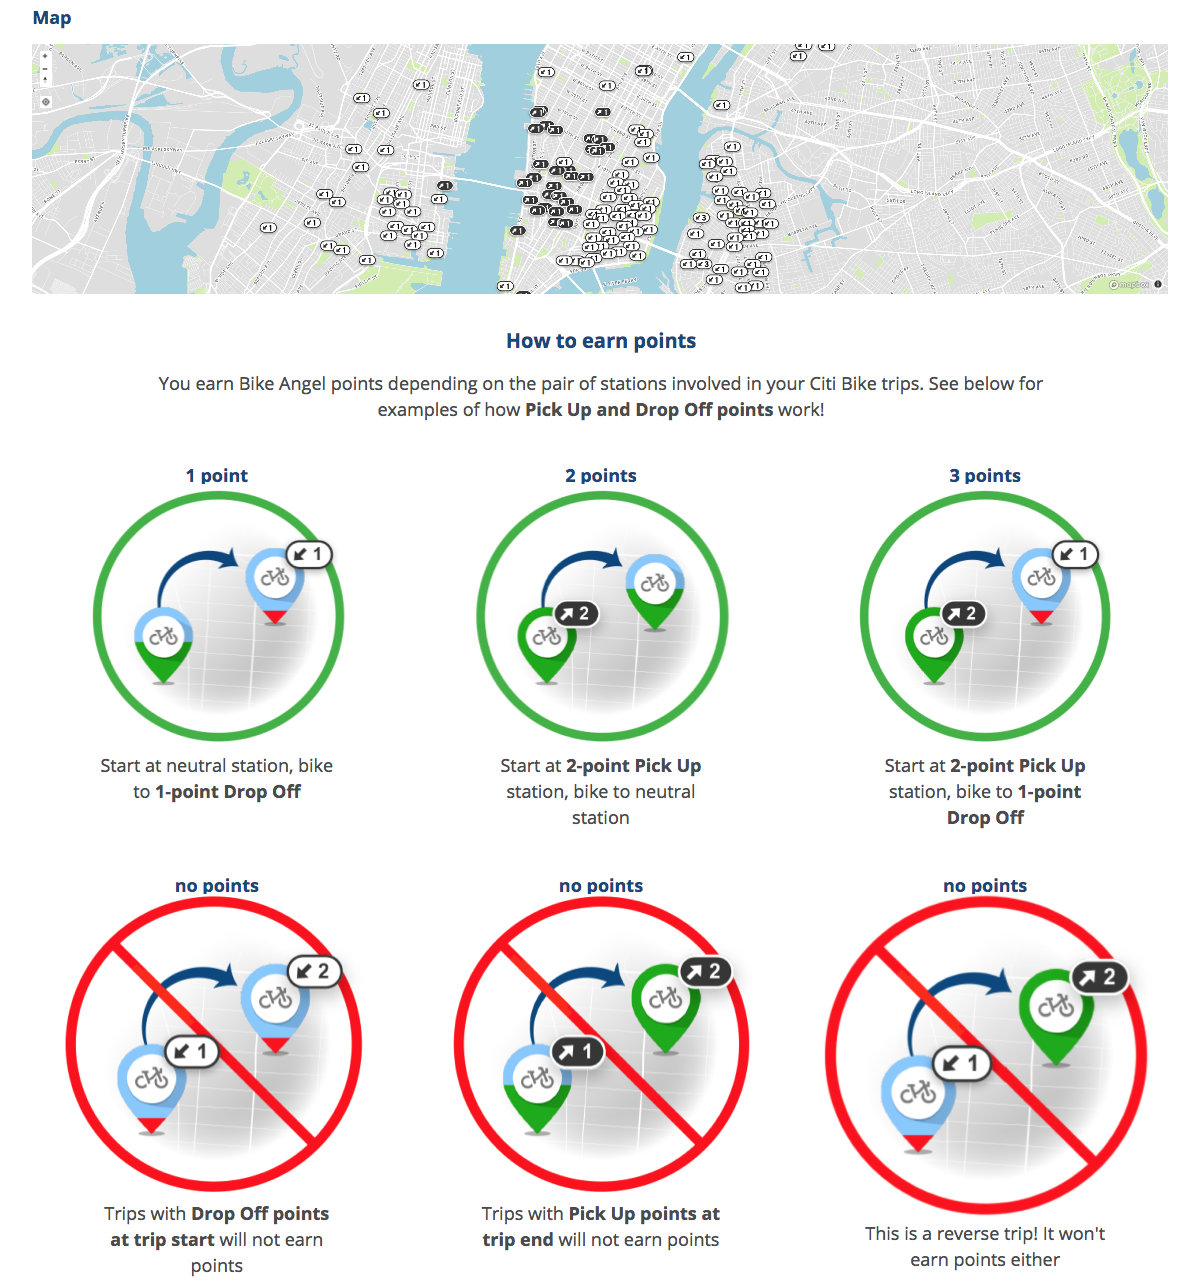
\includegraphics[width=.49\textwidth]{../Plots/screenshot_angels.png}
%\caption{Screenshot of Bike Angels website, displaying the dynamic map and explaining how to earn points.}
%\label{fig:screenshot_angels}
%\end{figure}
 %our work has had on the design of the Bike Angel program.

%Motivation is to understand when/how/where to use incentives to induce positive behavior

%Apply the standard BSS inventory model to Citi Bike's incentive scheme data

%Estimate the impact on out-of-stock events of each rental/return for which points where awarded

%Design different policies, distinguish between levels of static/dynamic

%Report on the influence on design in NYC

%\subsection{Related Work}

%Bike-sharing systems have become ubiquitous in American cities. Most of these systems are station-based, that is, they consist of a number of capacitated stations at which bikes can be rented or returned. The major operational challenge these systems face  is due to asymmetry in demand: stations in residential areas run out of bikes in the morning hours whereas the stations become full and then cannot have additional bikes returned.

%In this work, we investigate the impact of Citi Bike's incentive scheme. Referred to as \emph{Bike Angel} program, the incentive scheme was installed with our guidance in October 2015. A key feature of the incentive scheme, as suggested by \cite{OMahony2015}, is the categorization stations into ones at which rentals/returns are incentivized. Noticeably, labeling a station as a return station when such a station indeed has too few empty docks available can yield to outcomes in which the operator rewards, through the incentives,returns/rentals that have negative impact on the balance of the system.

%\subsection{Contribution} We apply a well-studied inventory model of bike-sharing stations to the problem of determining when to incentivize returns/rentals at stations. To do so, we compare the performance of various static and dynamic policies with respect to the estimated impact of incentivized trips on out-of-stock events. Additionally, we use predictive methods to estimate the probability of an incentivized trip occurring due to or independently of the incentives given. Thus, for a given cost parameter associated to each incentive point awarded, we find optimal subset of trips to incentivize.

%In order to accommodate practical constraints, we also investigate various different policies that are less dynamic in that decisions are made offline rather than on a minutely basis. We demonstrate the trade-offs between solution quality and online decision-making on Citi Bike's data-set, whilst also proving that in particular fluid sense, the optimal solution has a great deal of structure. Finally, we define a formal notion


